% =============================================================================
% ANALYSE DE LA LOI D'AMDAHL - GNU MAKE DISTRIBUÉ
% Projet Grenoble INP - Ensimag
% Généré automatiquement par amdahl_analysis.py
% =============================================================================

\documentclass[11pt,a4paper]{article}
\usepackage[utf8]{inputenc}
\usepackage[T1]{fontenc}
\usepackage[french]{babel}
\usepackage{amsmath,amssymb}
\usepackage{booktabs}
\usepackage{graphicx}
\usepackage{siunitx}
\usepackage{xcolor}

\begin{document}

% -----------------------------------------------------------------------------
% FORMULE CALIBRÉE
% -----------------------------------------------------------------------------
\section{Modèle Théorique Calibré}

Le modèle d'Amdahl modifié avec overhead de coordination:

\begin{equation}
\boxed{T(N) = T_{\text{seq}} + \frac{T_{\text{par}}}{N} + C \cdot \sqrt{N}}
\end{equation}

Avec les paramètres calibrés:

\begin{equation}
\boxed{T(N) = 15.00 + \frac{241.61}{N} + 0.50 \cdot \sqrt{N}}
\end{equation}

\begin{table}[h]
\centering
\caption{Paramètres du modèle calibré}
\begin{tabular}{lrl}
\toprule
\textbf{Paramètre} & \textbf{Valeur} & \textbf{Description} \\
\midrule
$T_{\text{seq}}$ & 15.00 s & Temps séquentiel incompressible \\
$T_{\text{par}}$ & 241.61 s & Temps total parallélisable \\
$C$ & 0.50 s & Coefficient d'overhead \\
\bottomrule
\end{tabular}
\end{table}

% -----------------------------------------------------------------------------
% MÉTRIQUES DE QUALITÉ
% -----------------------------------------------------------------------------
\section{Qualité du Modèle}

\begin{table}[h]
\centering
\caption{Métriques de qualité de l'ajustement}
\begin{tabular}{lr}
\toprule
\textbf{Métrique} & \textbf{Valeur} \\
\midrule
Coefficient de détermination ($R^2$) & 0.9906 \\
Erreur moyenne absolue (MAE) & 4.67 s \\
Erreur moyenne relative (MAPE) & 13.69 \% \\
Erreur quadratique moyenne (RMSE) & 5.34 s \\
\bottomrule
\end{tabular}
\end{table}

% -----------------------------------------------------------------------------
% DÉCOMPOSITION DU TEMPS
% -----------------------------------------------------------------------------
\section{Décomposition du Temps}

\begin{table}[h]
\centering
\caption{Décomposition du temps d'exécution}
\begin{tabular}{lrr}
\toprule
\textbf{Composante} & \textbf{Temps (s)} & \textbf{Proportion} \\
\midrule
Compilation & 6.00 & 40\% de $T_{\text{seq}}$ \\
Split (découpage) & 4.50 & 30\% de $T_{\text{seq}}$ \\
Merge (fusion) & 4.50 & 30\% de $T_{\text{seq}}$ \\
\midrule
\textbf{Total séquentiel} & \textbf{15.00} & \\
\midrule
20 tâches parallèles & 241.61 & 12.08 s/tâche \\
\bottomrule
\end{tabular}
\end{table}

% -----------------------------------------------------------------------------
% TABLEAU COMPARATIF COMPLET
% -----------------------------------------------------------------------------
\section{Résultats Détaillés}

\begin{table}[h]
\centering
\caption{Comparaison théorie vs expérimental}
\sisetup{round-mode=places, round-precision=2}
\begin{tabular}{r S[round-precision=2] S[round-precision=2] S[round-precision=1] S[round-precision=2] S[round-precision=1]}
\toprule
{$N$} & {$T_{\exp}$ (s)} & {$T_{\text{théo}}$ (s)} & {Erreur (\%)} & {Speedup} & {Eff. (\%)} \\
\midrule
1 & 262.39 & 257.11 & +2.0 & 1.00 & 100.0 \\
2 & 136.15 & 136.51 & -0.3 & 1.93 & 96.4 \\
3 & 91.18 & 96.40 & -5.7 & 2.88 & 95.9 \\
4 & 85.59 & 76.40 & +10.7 & 3.07 & 76.6 \\
5 & 65.02 & 64.44 & +0.9 & 4.04 & 80.7 \\
6 & 55.11 & 56.49 & -2.5 & 4.76 & 79.4 \\
7 & 48.79 & 50.84 & -4.2 & 5.38 & 76.8 \\
8 & 43.23 & 46.62 & -7.8 & 6.07 & 75.9 \\
9 & 40.19 & 43.35 & -7.9 & 6.53 & 72.5 \\
10 & 31.60 & 40.74 & -28.9 & 8.30 & 83.0 \\
11 & 31.55 & 38.62 & -22.4 & 8.32 & 75.6 \\
12 & 33.60 & 36.87 & -9.7 & 7.81 & 65.1 \\
13 & 30.13 & 35.39 & -17.5 & 8.71 & 67.0 \\
14 & 29.10 & 34.13 & -17.3 & 9.02 & 64.4 \\
15 & 27.71 & 33.04 & -19.2 & 9.47 & 63.1 \\
16 & 27.63 & 32.10 & -16.2 & 9.50 & 59.4 \\
17 & 27.04 & 31.27 & -15.7 & 9.70 & 57.1 \\
18 & 25.82 & 30.54 & -18.3 & 10.16 & 56.5 \\
19 & 20.06 & 29.90 & -49.0 & 13.08 & 68.8 \\
20 & 24.93 & 29.32 & -17.6 & 10.53 & 52.6 \\
\bottomrule
\end{tabular}
\end{table}

% -----------------------------------------------------------------------------
% ANALYSE
% -----------------------------------------------------------------------------
\section{Analyse}

\begin{itemize}
    \item \textbf{Fraction séquentielle:} $f = T_{\text{seq}} / T(1) = 5.7\%$
    \item \textbf{Fraction parallèle:} $1-f = 94.3\%$
    \item \textbf{Speedup maximum théorique:} $S_{\max} = 1/f = 17.49$
    \item \textbf{Speedup observé à N=20:} $S_{20} = 10.53$
    \item \textbf{Efficacité moyenne:} 73.3\%
\end{itemize}

% Figure
\begin{figure}[h]
\centering
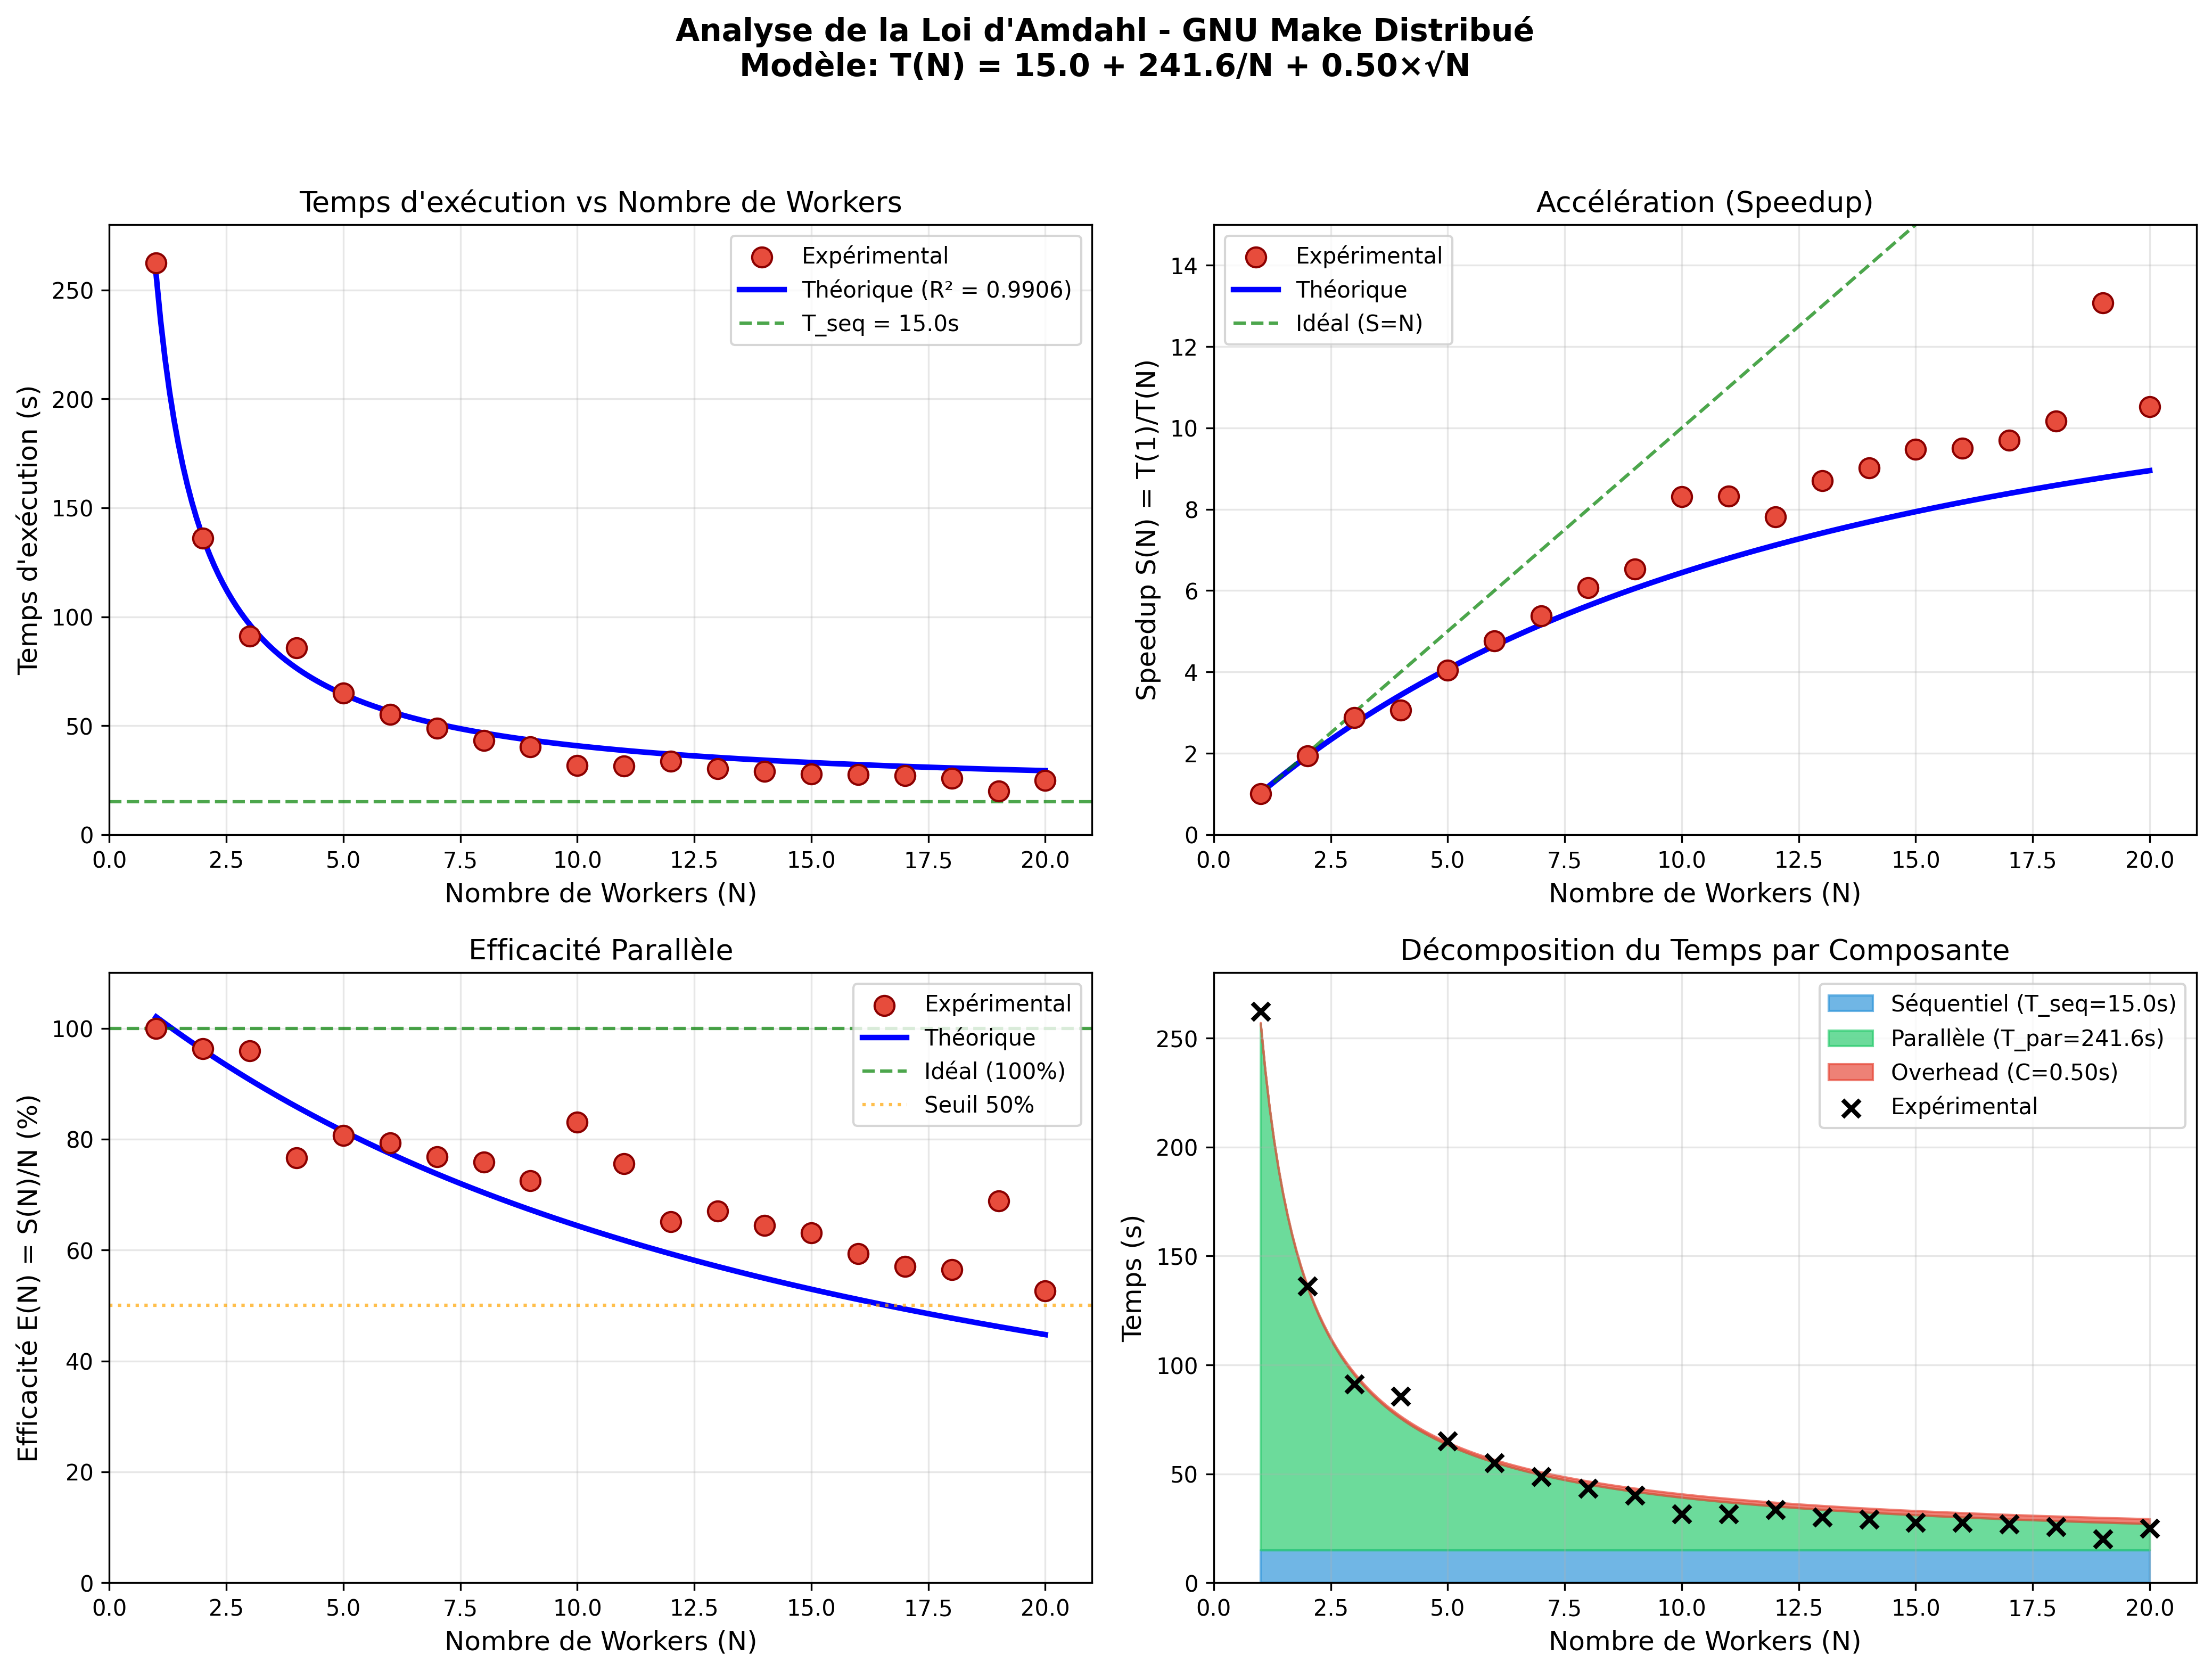
\includegraphics[width=\textwidth]{amdahl_analysis.png}
\caption{Analyse complète de la loi d'Amdahl}
\end{figure}

\end{document}
